\documentclass{article}
\usepackage{amsmath, amssymb}
\usepackage{graphicx}
\usepackage[margin=1.0in]{geometry}  % Set all margins to 1 inch

\title{Stochastic update steps for sharply calibrating binary statistics}

\begin{document}
\maketitle

\begin{abstract}
The documents describes and provides some preliminary results for a new stochastic parameter update for calibrating generative models to shift the mean of binary statistics.
The motivation is that the unbiased gradient estimates obtainable from a squared error violation loss decay too aggressively as a model approaches the target mean, because the magnitude of gradient estimates scale linearly with the Monte Carlo estimate of the size of the constraint violation.
So we explore an update that removes this linear scaling.
The update resembles a Monte Carlo estimate of the gradient of the absolute error (rather than squared error) loss, but unlike a naive gradient of absolute error is scaled in a way that maintains convergence to the desired expectation.
\end{abstract}


\paragraph{Setting and notation:}
\begin{itemize}
    \item Generative model $p_\theta(x)$
    \item \textit{Binary} statistic $h(x) \in \{0, 1\}$
    \item Target value $h^* \in [0, 1]$
\end{itemize}

For fine-tuning with current version of CGM relax our procedure looks like this
\begin{enumerate}
    \item sample $x_1, \dots, x_M \overset{iid}{\sim} p_\theta,$
    \item compute $y = \frac{1}{M}\sum h(x_m),$ and
    \item update $\theta$ by taking a descent step $\theta \leftarrow \theta - \alpha\,\hat U(\theta, x_{1:M})$, where
    \[
        \hat U(\theta, x_{1:M}) = \left[\frac{1}{M}\sum (\nabla_\theta \log p_\theta(x_m))w(h(x_m))\right] \eta(y).
    \]
\end{enumerate}

\paragraph{Squared error.}
\begin{itemize}
    \item The squared error corresponds to choosing $w(h) = h - h^*$, so $w(0) = -h^*$ and $w(1) = 1 - h^*$, and $\eta(y) = 2(y - h^*)$.
    \item When $y < h^*$, $\eta(y) < 0$, so $w(h(x_m))\eta(y)$ is negative for $h(x_m)=1$ and positive for $h(x_m)=0$. The descent step $\theta \leftarrow \theta - \alpha\hat U$ therefore increases the likelihood of samples with $h(x_m)=1$ and decreases it for $h(x_m)=0$, pushing $\mathbb{E}_\theta[h(x)]$ toward $h^*$.
    \item We also add a bias correction so that $\hat U$ is an unbiased estimator of the negative gradient of the squared error, $\nabla_\theta (\mathbb{E}_\theta[h(x)] - h^*)^2$, so the descent step reduces the squared calibration error in expectation. Deriving the bias correction is possible because of a bias-variance decomposition special to the squared error.
    \item However, a limitation of this loss is that the violation doesn't become small enough. Reason: the magnitude of the expected gradient is too small near $h^*$. We regularly see optimization stop short of satisfying the constraint.
\end{itemize}

\paragraph{Absolute error.}
An alternative approach is to define
\[
    \hat U(\theta, x_{1:M}) = \nabla_\theta \left|\frac{1}{M}\sum \frac{p_{\theta}(x_m)}{p_{\mathrm{SG}(\theta)}} h(x_m) - h^*\right|.
\]
This resembles an gradients of the absolute loss loss that we might hope to better guarantee exact satisfaction of the constraint. But it is not clear how to make it unbiased. And in particular it has the disadvantage that the value of the gradient estimator will almost surely be identical for every $h^* \in (0, \frac{1}{M})$. Consequently, the approach will not be able to distinguish frequencies of rare events with probability below $\frac{1}{M}$.

\paragraph{Stationary REINFORCE.}
We would like to choose another (stochastic) update direction that has expectation zero when $\mathbb{E}_\theta[h(x)] = h^*$. We consider
\[
    \hat U(\theta, x_{1:M}) = \left[\frac{1}{M}\sum (\nabla_\theta \log p_\theta(x_m))w(h(x_m))\right] \cdot (-1)^{\mathbb{I}[y < h^*]}
\]
with
\[
    w(0) = \frac{-(1-h^*)(h^* - 2\alpha\beta)}{D}, \qquad w(1) = \frac{h^*\bigl(2\alpha(1-\beta)-(1-h^*)\bigr)}{D}, \qquad D = 2\alpha(h^* - \beta),
\]
where $\alpha$ and $\beta$ relate to statistics of the binomial distribution and depend on $h^*$ and the batch size $M$. 
\begin{itemize}
    \item Let $y \in \{0, \tfrac{1}{M}, \dots, 1\}$ be the empirical fraction with $y = Z/M$ and $Z \sim \mathrm{Binomial}(M, h^*)$.
    \item Define $\alpha = P\!\left[y < h^*\right]$. 
    \item Define $\beta = \mathbb{E}\!\left[y \mid y < h^*\right]$.
    \item \textit{Intuition:} For samples with $h(x_m) = 0$, a descent step decreases the probability of $x_m$ if $y < h^*$. With $y < h^*$, the factor in front of $\nabla_\theta \log p_\theta(x_m)$ in $\hat U$ is $+1$, and so a descent step is in the direction $-\nabla_\theta \log p_\theta(x_m)$.
\end{itemize}

\paragraph{Claim:} If $\mathbb{E}_\theta[h(x)] = h^*$, then $\mathbb{E}_\theta[\hat U(\theta, x_{1:M})] = 0$.



\textit{Proof.} By the law of total expectation, letting $y = \frac{1}{M}\sum h(x_m)$:
\begin{align*}
\mathbb{E}_{\theta}[\hat U(\theta, x_{1:M})]
    &= P_\theta[y < h^*]\, \mathbb{E}_\theta\!\left[M^{-1}\sum w(h(x_m))\nabla_\theta \log p_\theta(x_m) \mid y < h^*\right](-1) \\
    &\quad + P_\theta[y \ge h^*]\, \mathbb{E}_\theta\!\left[M^{-1}\sum w(h(x_m))\nabla_\theta \log p_\theta(x_m) \mid y \ge h^*\right].
\end{align*}
Letting $\alpha = P_\theta[y < h^*]$:
\begin{align*}
    &= -\alpha\, \mathbb{E}_\theta\!\left[M^{-1}\sum w(h(x_m))\nabla_\theta \log p_\theta(x_m) \mid y < h^*\right] \\
    &\quad + (1-\alpha)\, \mathbb{E}_\theta\!\left[M^{-1}\sum w(h(x_m))\nabla_\theta \log p_\theta(x_m) \mid y \ge h^*\right].
\end{align*}
Letting $s_i = \mathbb{E}_\theta[\nabla_\theta \log p_\theta(x) \mid h(x) = i]$, $\beta = \mathbb{E}_\theta[y \mid y < h^*]$, and $\gamma = \mathbb{E}_\theta[y \mid y \ge h^*]$:
\begin{align*}
    &= -\alpha\big[w(1)\beta s_1 + w(0)(1-\beta)s_0\big] + (1-\alpha)\big[w(1)\gamma s_1 + w(0)(1-\gamma)s_0\big].
\end{align*}
Replacing $\gamma = \frac{h^* - \alpha\beta}{1-\alpha}$ and $s_1 = -\frac{1-h^*}{h^*}s_0$, and collecting terms in $s_0$:
\begin{align*}
    &= \left[w(1)\frac{1-h^*}{h^*}(h^*-2\alpha\beta) + w(0)\bigl(1-2\alpha(1-\beta)-h^*\bigr)\right](-s_0).
\end{align*}
Substituting $w(1) = h^*(2\alpha(1-\beta)-(1-h^*))/D$ and $w(0) = -(1-h^*)(h^*-2\alpha\beta)/D$:
\begin{align*}
    &= \frac{1-h^*}{D}\left[(2\alpha(1-\beta)-(1-h^*))(h^*-2\alpha\beta) - (h^*-2\alpha\beta)(2\alpha(1-\beta)-(1-h^*))\right](-s_0) = 0.\qquad\square
\end{align*}

\textbf{Implementation note:} A naive implementation can lead to numerical issues.  We remark on these issues and a solution.
\begin{itemize}
    \item Both numerators are positive provided $M$ is not too large relative to $1/h^*$ ($D > 0$ always since $\beta < h^*$).
    \item When the numerator of $w(1)$ is non-positive---which occurs when $M$ is large and few discrete outcomes fall below $h^*$, so $\alpha$ is small---the finite-$M$ formula is invalid because it would yield $w(1)\le 0$, reversing the update direction.
    \item In this regime $D$, $h^*-2\alpha\beta$, and $2\alpha(1-\beta)-(1-h^*)$ all vanish at the same $O(\sigma)$ rate as $M\to\infty$ (CLT, $\sigma=\sqrt{h^*(1-h^*)/M}$).
    \item By L'H\^{o}pital's rule the weights converge to $w(0)\to -(1-h^*)$, $w(1)\to h^*$, which are used as the fallback.
    \item The normalization $D$ is chosen so that $w(1) - w(0) = 1$, matching the absolute-error gradient scaling for $p$ far from $h^*$, for any $M$.
    \item An advantage of this construction is that the weights are also symmetric under $h^* \leftrightarrow 1-h^*$ (the roles of $w(0)$ and $w(1)$ swap), and recover $w(1) \to h^*$, $w(0) \to -(1-h^*)$ as $M \to \infty$.
\end{itemize}

\paragraph{Comparison of estimators.}
Figure~\ref{fig:implied_loss} compares the three estimators on a Bernoulli$(p)$ model with $h(x)=x$, so $\mathbb{E}_\theta[h(x)] = p$.
The top row shows the expected update direction $\mathbb{E}_p[\hat{U}]$ as a function of the model parameter $p$, for four target values $h^*$.
The bottom row shows the \emph{implied loss} $V(p) = \int_0^p \mathbb{E}_q[\hat{U}]\,/\,(q(1-q))\,\mathrm{d}q$ (shifted so $V(h^*)=0$), which is the loss whose gradient the update direction corresponds to in parameter space.

All three estimators satisfy $\mathbb{E}_{h^*}[\hat{U}] = 0$, confirming stationarity at $p = h^*$.
The squared error estimator has an implied loss equal to $(p - h^*)^2$ and its expected gradient decays quadratically near $h^*$, which can cause optimization to stall.
The absolute error and Stationary REINFORCE estimators have implied losses that are approximately $V$-shaped near $h^*$, with gradients that remain bounded away from zero, leading to sharper convergence near the constraint.
Batch size $M=32$ is used to ensure the Stationary REINFORCE formula is valid across all $h^*$ values shown.

\begin{figure}[h]
    \centering
    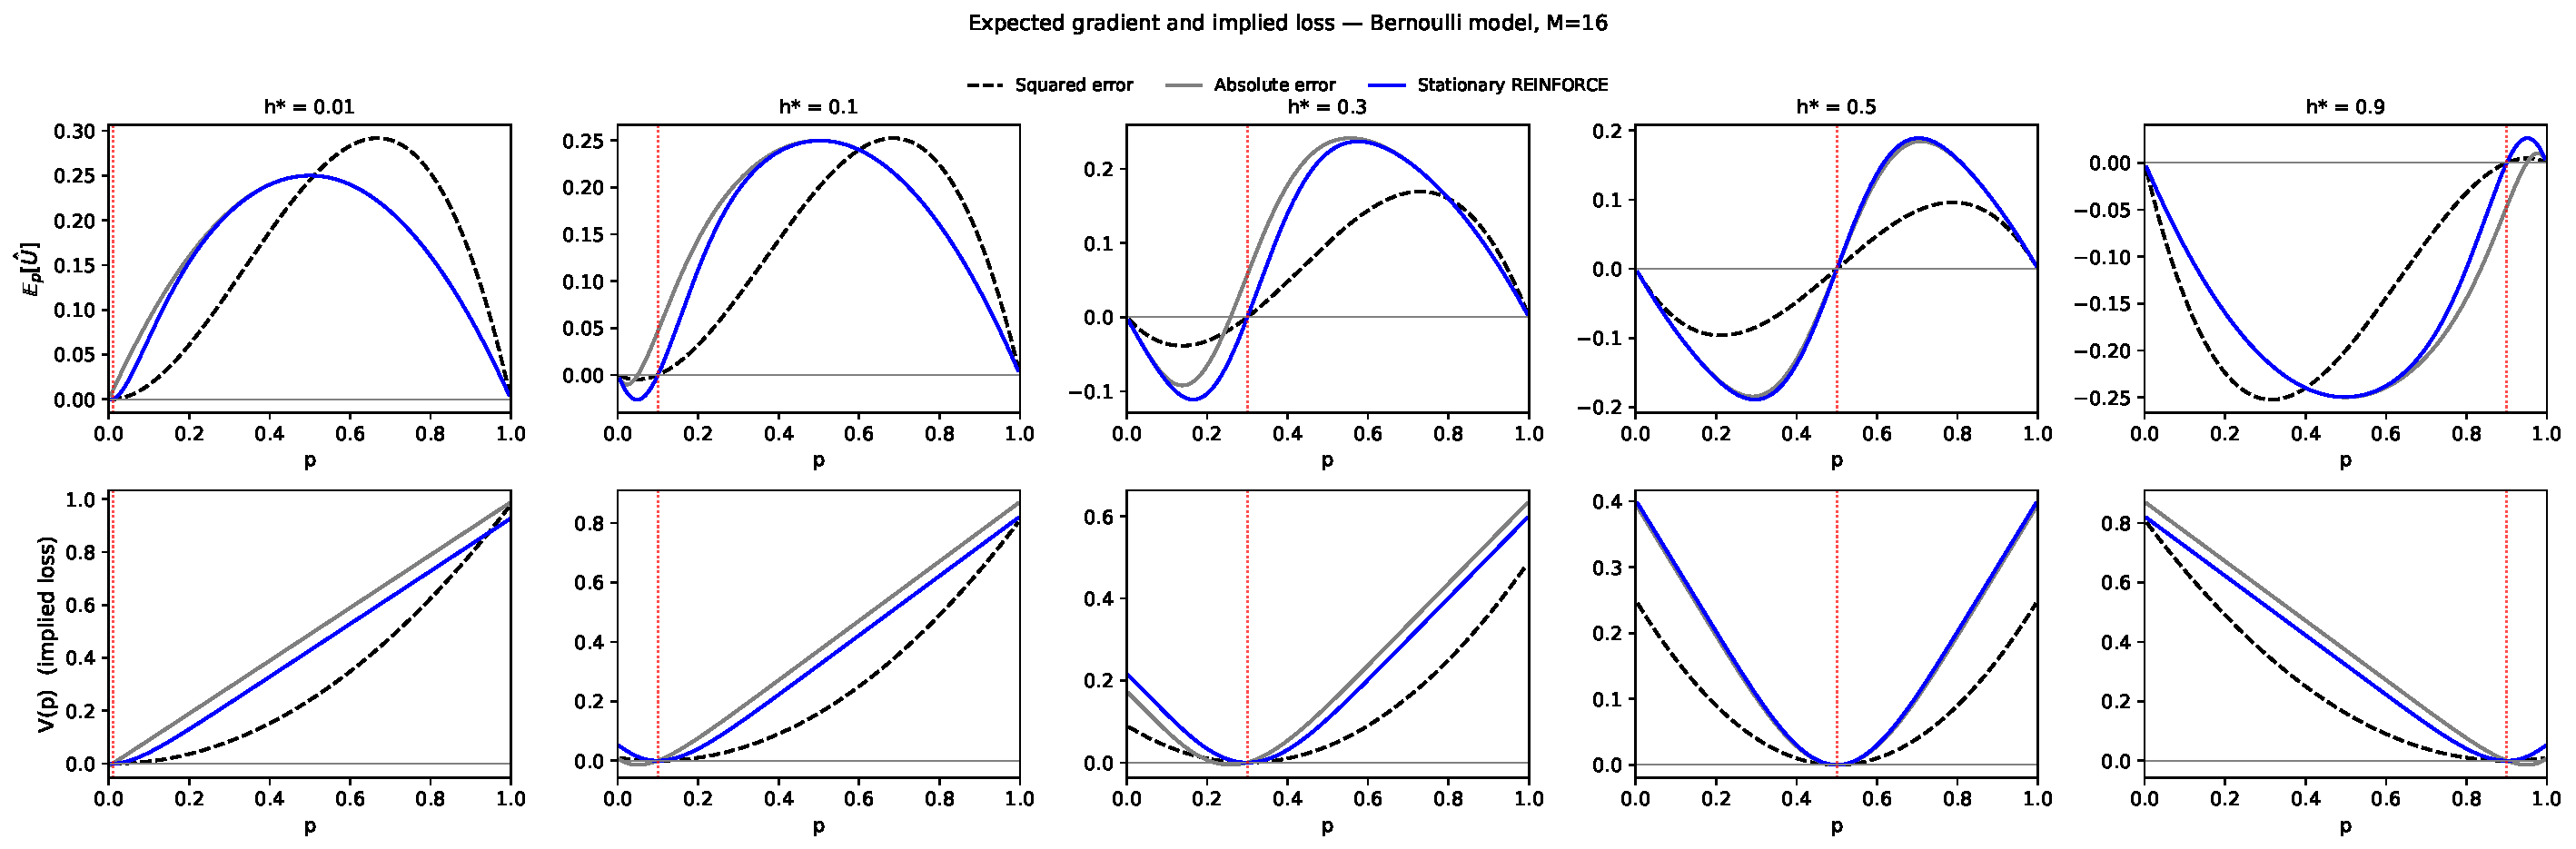
\includegraphics[width=\textwidth]{./sr_analysis.pdf}
    \caption{%
        \textbf{Expected update direction and implied loss for three estimators on the Bernoulli model.}
        Top: $\mathbb{E}_p[\hat{U}]$ vs.\ model parameter $p$ for target values $h^* \in \{0.1, 0.3, 0.5, 0.9\}$ and batch size $M=32$.
        Bottom: implied loss $V(p) = \int_0^p \mathbb{E}_q[\hat{U}]\,/\,(q(1-q))\,\mathrm{d}q$, shifted so $V(h^*)=0$.
        The dashed red line marks $p = h^*$.
        All three estimators have zero expected update at $p = h^*$
        The Stationary REINFORCE and absolute error estimators maintain larger gradients near $h^*$ compared to the squared error baseline.
    }
    \label{fig:implied_loss}
\end{figure}

\paragraph{Bernoulli calibration experiment.}
Figure~\ref{fig:bernoulli_comparison} compares Squared Error and Stationary REINFORCE on a Bernoulli$(p)$ model, initialized at $p=0.5$ and calibrated to a target $h^*$ using gradient descent on $\theta = \mathrm{logit}(p)$.
We vary $h^* \in \{0.1, 0.01, 0.001\}$ and batch size $M \in \{8, 32, 128\}$, running 4 independent replicates of 5000 gradient steps each with learning rate $3\times10^{-2}$ and Adam optimizer.
Calibration error $|\mathbb{E}_{p_\theta}[h(x)] - h^*|$ is estimated every 10 steps using 10{,}000 samples.

The results show a clear qualitative difference between the two methods that becomes more pronounced as $h^*$ decreases.
For $h^* = 0.1$, both methods converge to a similar floor around $10^{-2}$--$10^{-3}$, with Stationary REINFORCE converging faster in early iterations but showing higher variance at later steps.
For $h^* = 0.01$, Stationary REINFORCE consistently reaches lower calibration error, converging roughly an order of magnitude below the Squared Error baseline across all batch sizes.
For $h^* = 0.001$, the advantage is most dramatic: Stationary REINFORCE continues to drive the error toward $10^{-4}$ while Squared Error stalls at $10^{-3}$--$10^{-2}$, consistent with the theoretical prediction that the squared error gradient vanishes quadratically near $h^*$.
Larger batch sizes generally reduce variance but do not close the gap between methods.

\begin{figure}[h]
    \centering
    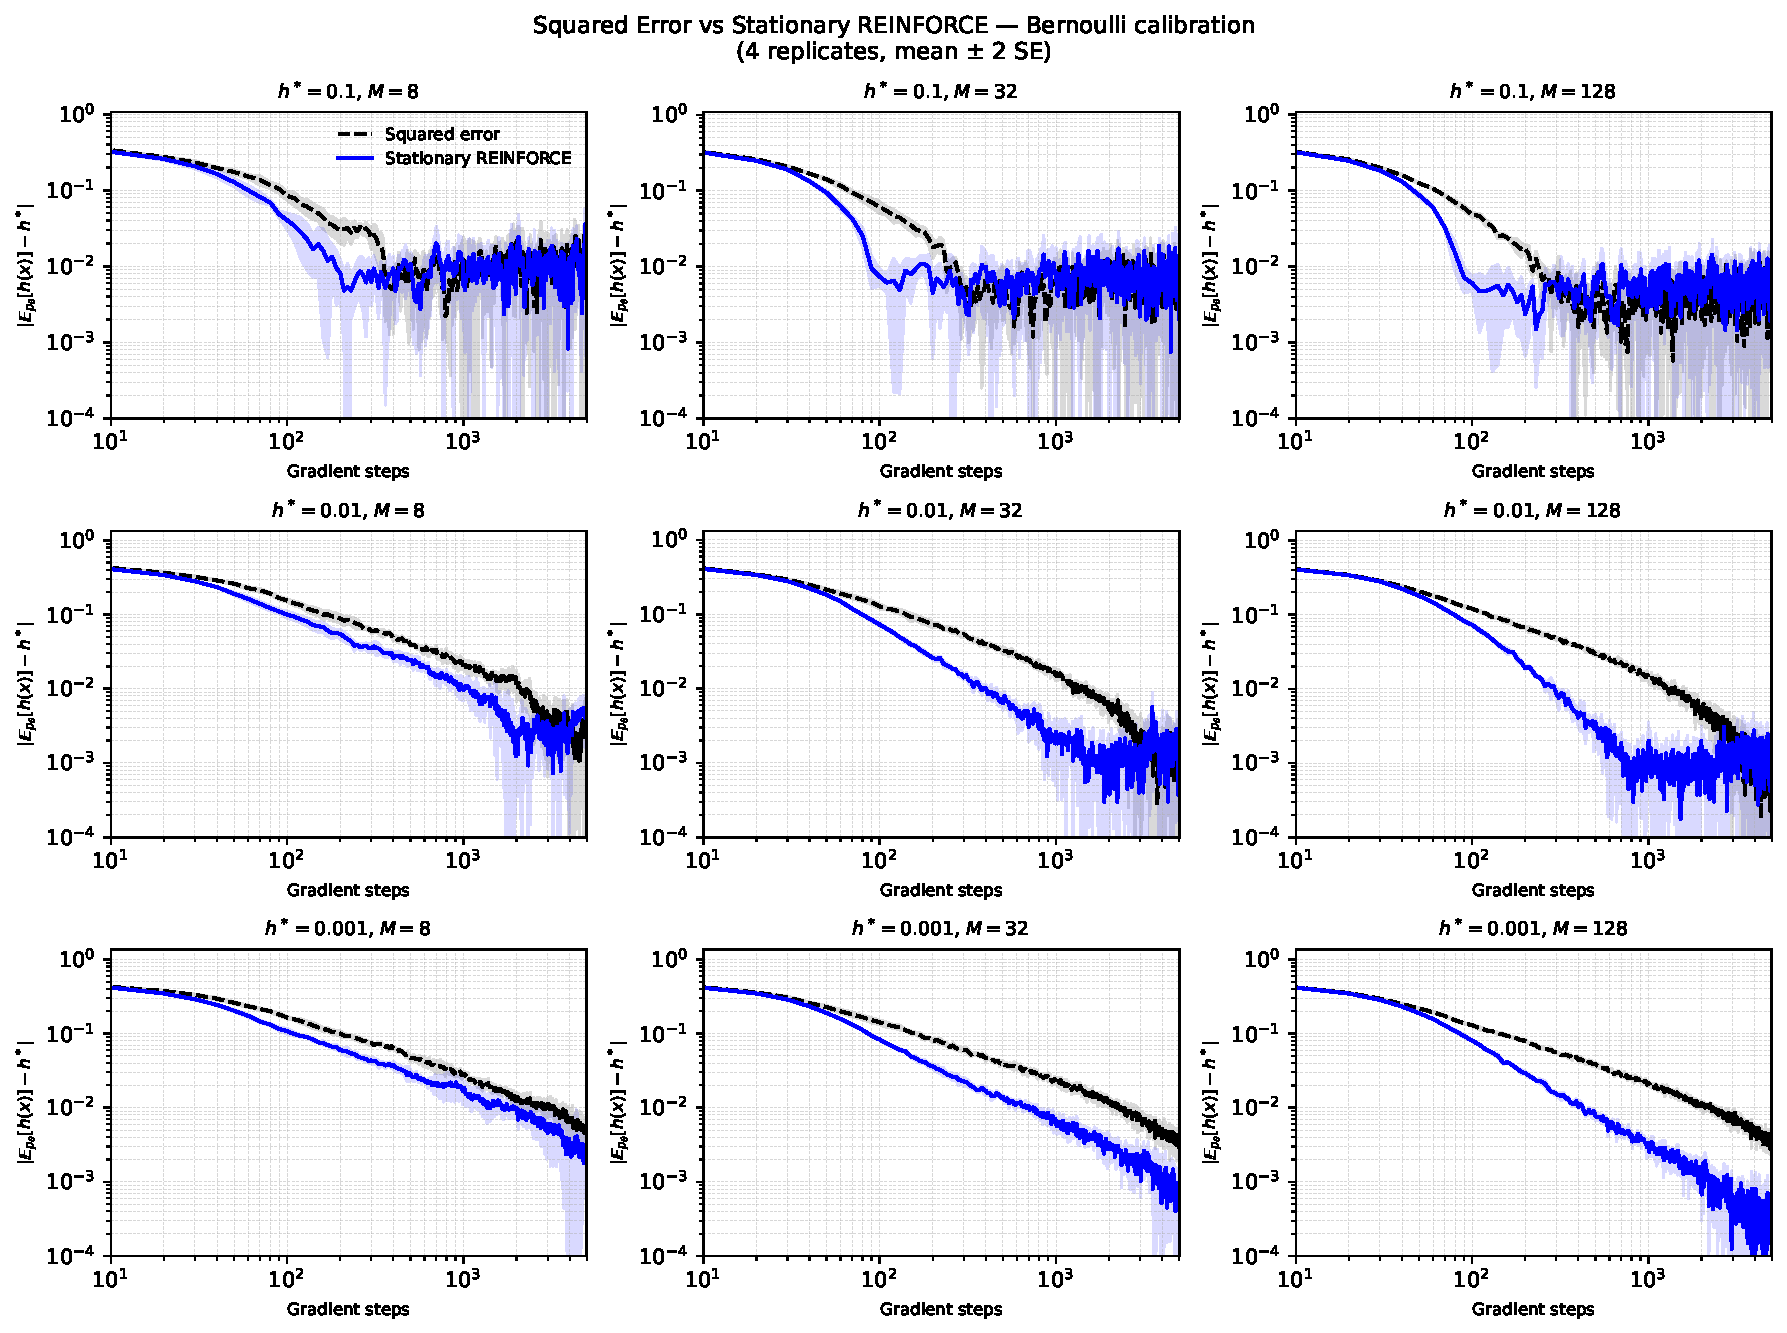
\includegraphics[width=\textwidth]{./bernoulli_comparison.pdf}
    \caption{%
        \textbf{Calibration error vs.\ gradient steps for Squared Error and Stationary REINFORCE on the Bernoulli model.}
        Each panel shows $|\mathbb{E}_{p_\theta}[h(x)] - h^*|$ on a log--log scale for a given target $h^*$ (rows) and batch size $M$ (columns).
        Curves show the mean over 4 replicates; shaded bands show $\pm 2$ standard errors.
        Stationary REINFORCE (blue) converges to lower calibration error than Squared Error (black dashed), with the advantage growing as $h^*$ decreases.
    }
    \label{fig:bernoulli_comparison}
\end{figure}

\end{document}
